\identify{Identify the Challenge \& Set Goals: Intake V1.0 (July 13, 2024)}
\chapterauthor{Caleb Bachmeier}
\textbf{Goal}: We will identify an objective for our robot so that we can address it and build an effective solution
\section*{Problem Statement}
We need a mechanism to put rings onto mobile goals and alliance stakes
\section*{Solution Requirements}
\begin{itemize}
    \item Must use legal VEX parts 
    \item Must be under 18 inches 
\end{itemize}
\section*{Solution Goals}
\begin{itemize}
    \item We would like to be able to expand into a redirect system (more on this later)
\end{itemize}
\brainstorm{Brainstorm \& Diagram: Intake V1.0 (July 15, 2024)}
\chapterauthor{Caleb Bachmeier}
\info{Caleb Bachmeier}{Brainstorm \& Diagram: Intake}{July 15, 2024}
\textbf{Goal}: Brainstorm possible solutions for an intake
\section*{Possible Solution - Intake}
\noindent
\textbf{Hook}:

A Hook intake is one of the two major Ring intake systems in High Stakes. A Hook system uses, unsurprisingly, a hook that picks up Rings of the ground, and flips them over into the Mobile Goal that is clamped down. This is shown more \href{https://www.youtube.com/watch?v=ybP6bGynbs4&t=5s}{in this prototype} built by Evan Rogerson, @9MotorGang on YouTube. \\
\noindent
\textbf{Pros}:
\begin{itemize}
    \item Quickly collects multiple rings, even while the robot is moving.
    \item Keeps rings aligned throughout the intake process to reduce jamming.
    \item Requires minimal adjustments once tuned properly.
    \item Can be converted into a redirect later on.
    \item Simple to build.
\end{itemize}

\textbf{Cons}:
\begin{itemize}
    \item May take up significant space within the robot's design constraints.
    \item Sharing motors with other mechanisms can complicate control.
    \item Requires precise roller speed and spacing to prevent jams.
    \item Takes up a lot of space.
\end{itemize}
\noindent
\textbf{Hood}:
A curved intake system that uses spinning rollers to collect rings and guide them upward smoothly.

\noindent
\textbf{Pros}:
\begin{itemize}
    \item Quickly collects multiple rings, even while the robot is moving.
    \item Keeps rings aligned throughout the intake process to reduce jamming.
    \item Requires minimal adjustments once tuned properly.
\end{itemize}

\textbf{Cons}:
\begin{itemize}
    \item May take up significant space within the robot's design constraints.
    \item Sharing motors with other mechanisms can complicate control.
    \item Requires precise roller speed and spacing to prevent jams.
\end{itemize}


\solution{Choose a Solution: Intake V1.0 (August 8th, 2024)}
\info{Connor Albers}{Intake V1.2}{August 8th, 2024}
\chapterauthor{Connor Albers}
\section*{Choose a Solution}
We reviewed several Intake concepts and decided to move forward with a multi-stage Intake inspired by \textit{7686B's} "\cite{7686b}"  floating Intake design from Spin Up. The multi-stage system allows for better Ring management and scoring efficiency. Below is a decision matrix that justifies our selection:

\renewcommand{\arraystretch}{1.85} % Change this value as needed
\begin{table}[htb!]
\centering
\begin{tabular}{|>{\centering\arraybackslash}m{1.85cm}|>{\centering\arraybackslash}m{1.85cm}|>{\centering\arraybackslash}m{1.85cm}|>{\centering\arraybackslash}m{1.85cm}|>{\centering\arraybackslash}m{1.85cm}|>{\centering\arraybackslash}m{1.85cm}|>{\centering\arraybackslash}m{1.85cm}|}
\hline
\textbf{Scale 1 - 10} & \textbf{Efficiency} & \textbf{Complexity} & \textbf{Ring Management} & \textbf{Motor Usage} & \textbf{Total} \tabularnewline
\hline
Weight & x3 & x2 & x3 & x2 & \tabularnewline
\hline
Hook Intake & 9 & 7 & 10 & 8 & 87 \tabularnewline
\hline
Single Stage Intake & 6 & 8 & 5 & 10 & 69 \tabularnewline
\hline
Floating Intake & 10 & 6 & 9 & 8 & 85 \tabularnewline
\hline
\end{tabular}
\caption{Intake V1.2 Decision Matrix}
\label{tab:Intake-v1.2-decision-matrix}
\end{table}
\renewcommand{\arraystretch}{1.85} % Reset to default

\section*{Make a Plan}
This solution involved a generic hook style Intake as shown in the basic design built by Evan Rogerson from the Vex U team JHAWK
\begin{figure}[H] 
\centering 
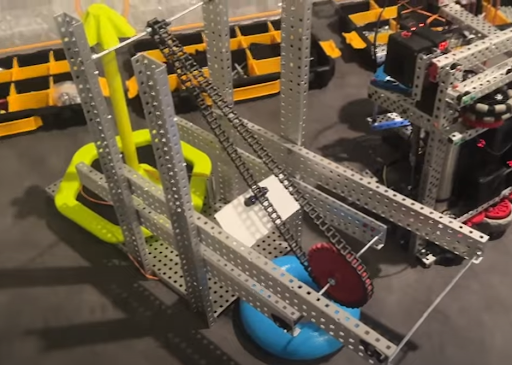
\includegraphics[width=0.5\linewidth]{images/9MotorGangHook.jpg} 
\caption{Evan Rogerson Hook Intake} 
\end{figure} 
with a one way flap in the middle of the chain section. 
\begin{figure}[H] 
\centering 
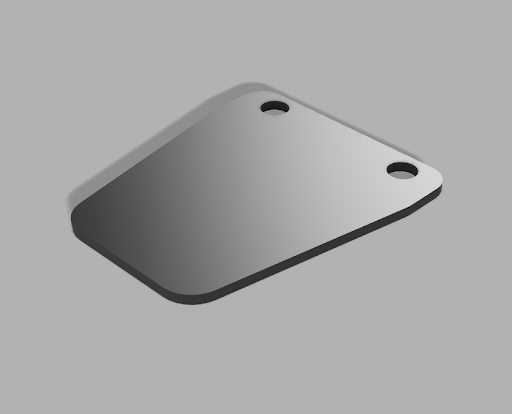
\includegraphics[width=0.5\linewidth]{images/Iso-hook-V1.png} 
\caption{CAD of a flap design} 
\end{figure} 

This flap would allow Rings forward, to be scored on a Mobile Goal but if the Intake was spun so that the Ring passed the flap and then the Intake was spun backwards the Ring would slide down a ramp and fall into a hopper. This solution allowed the use of the Intake, a more effective pick up system, to load an arm with Rings. With the first problem with a traditional hook style solved, the second issue was power. We needed a way to overcome the friction that comes along with having a two stage Intake. The solution we came up with was simple: we use two motors on the Intake as opposed to one, then to actuate the arm we would use pneumatics. 

\build{Build \& Program: Intake V1.0 (August 10th, 2024)}
\info{Connor Albers}{Intake V1.2}{August 10th, 2024}
\chapterauthor{Connor Albers}
\section*{Building}
With the key problems solved, it was time to start building. After disassembling the old four bar mechanism we were left with the two vertical towers. Luckily we could make use of these in the new design but that would come later; our first step was to create the first stage of the Intake. This portion of the build was inspired by \textit{7686B's} "\cite{7686b}" “floating” Intake from Spin Up 
\begin{figure}[H]
    \centering
    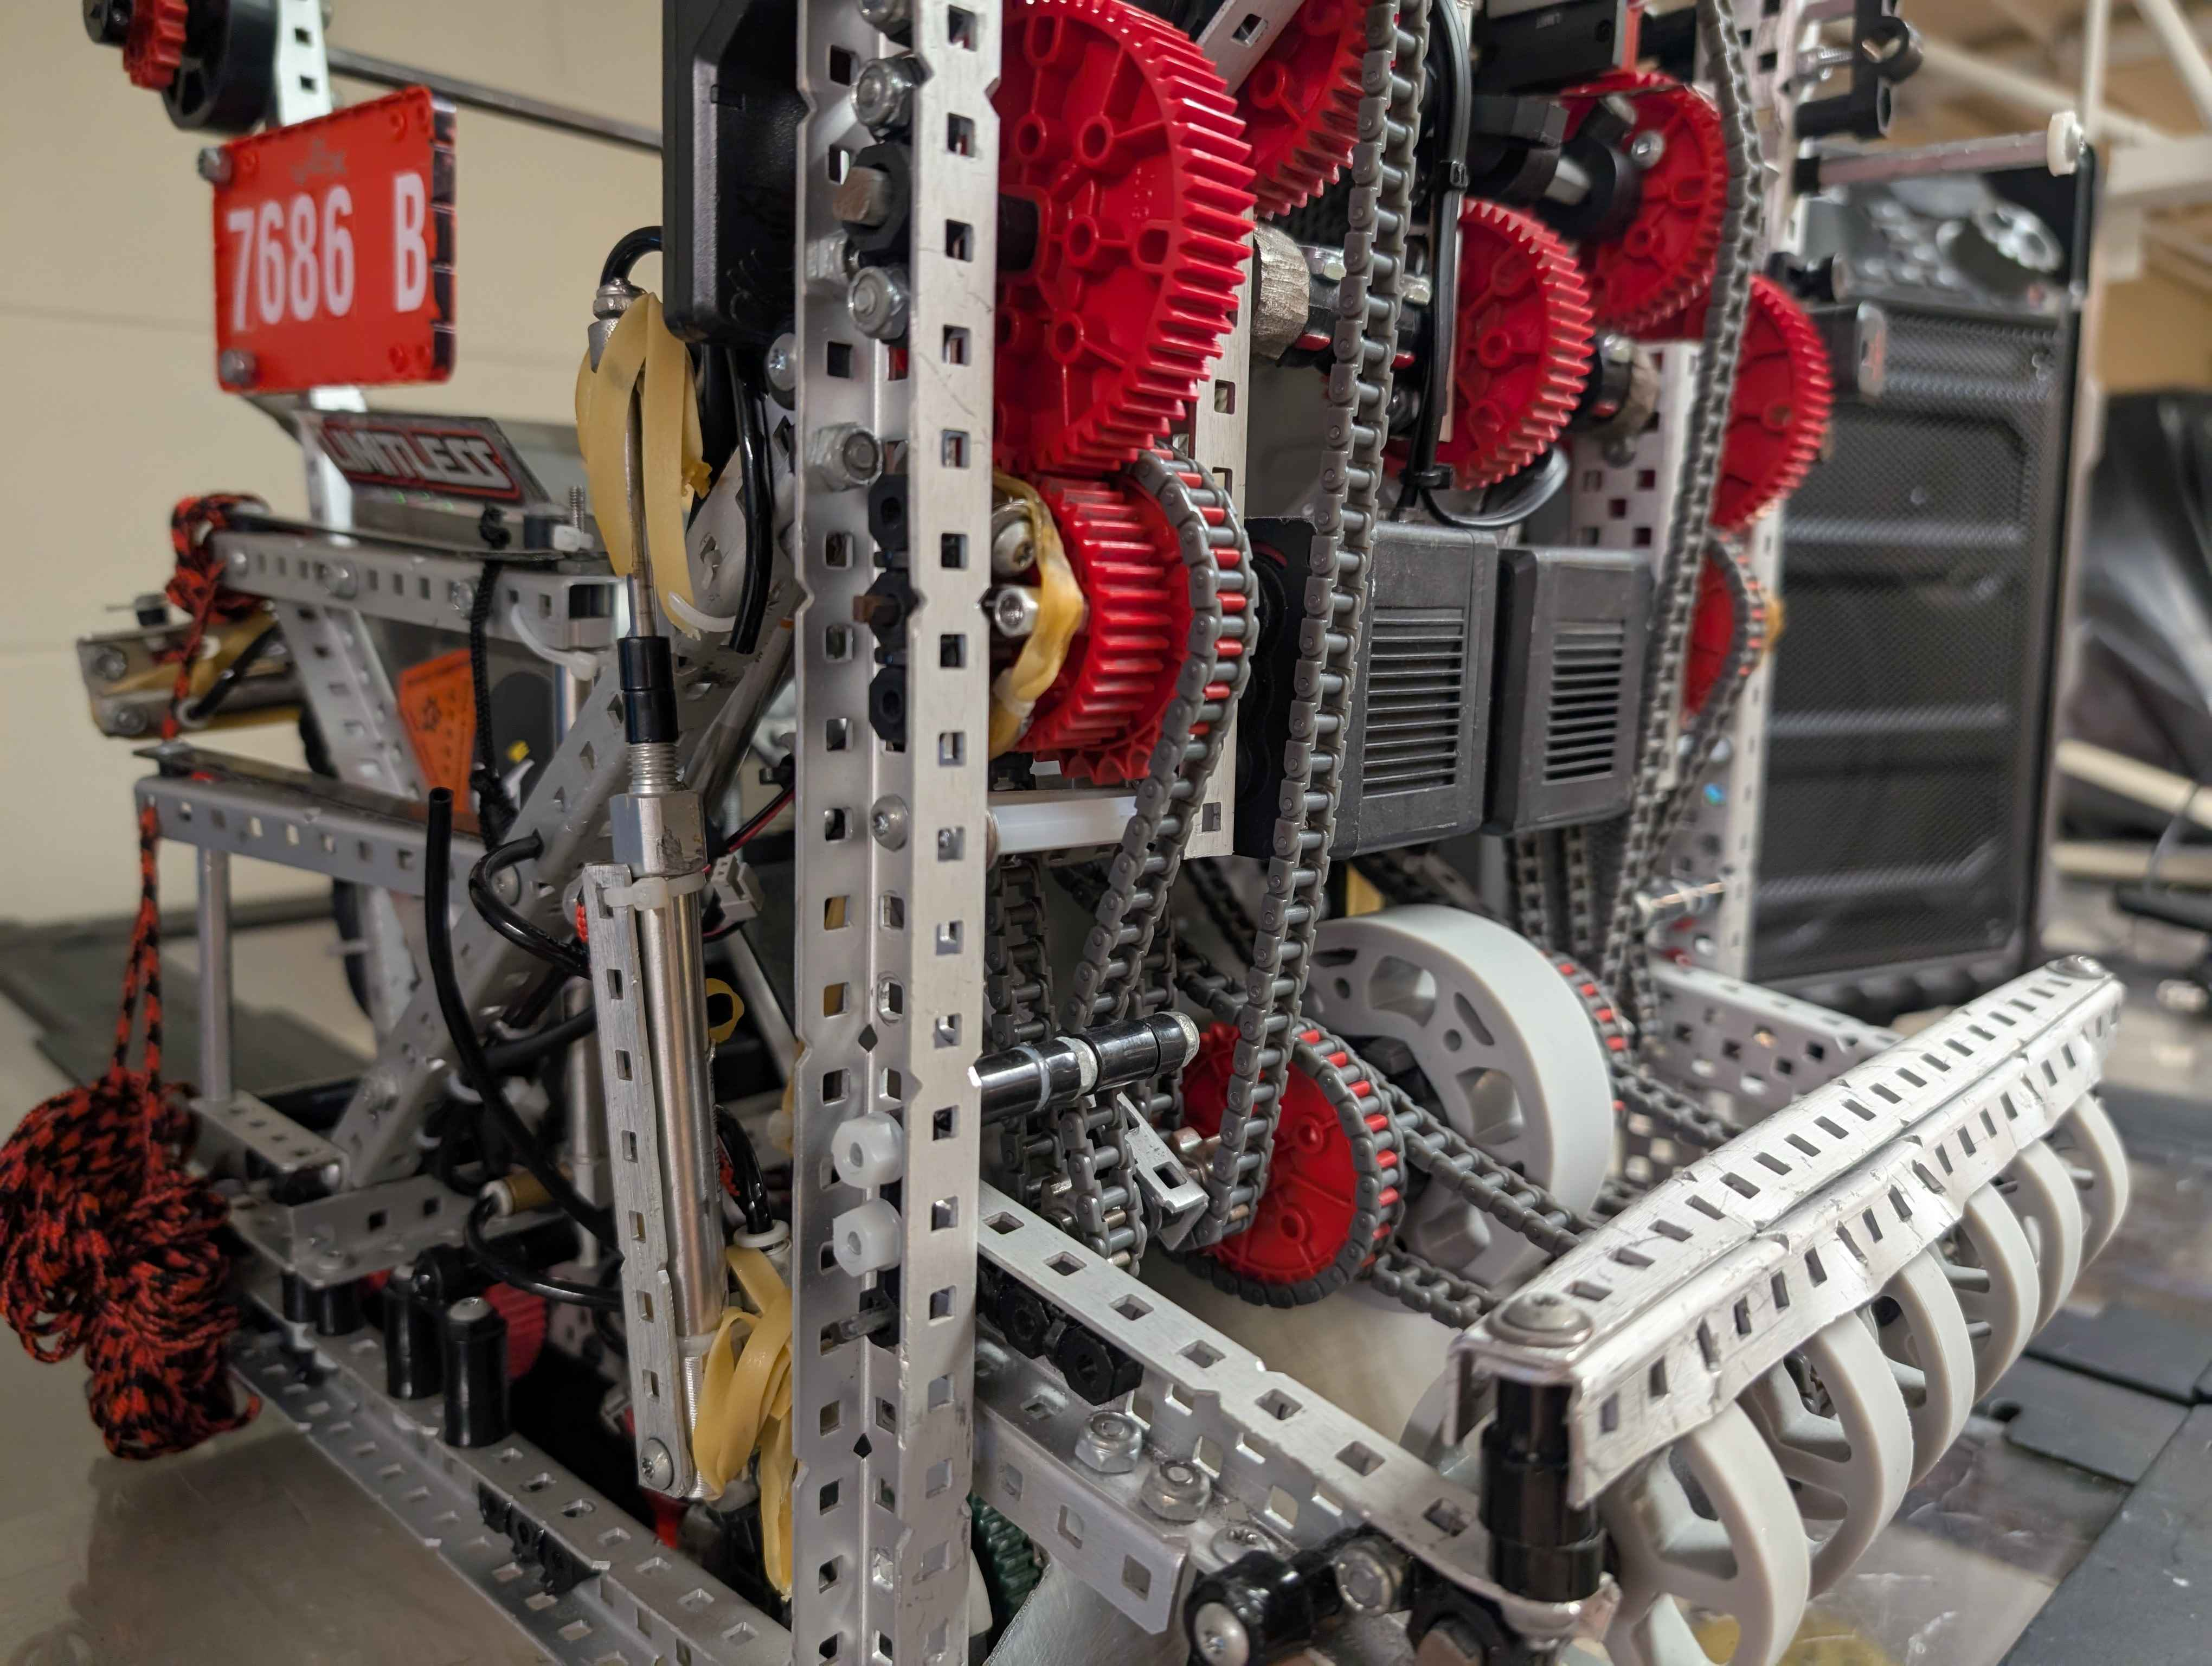
\includegraphics[width=0.5\linewidth]{images/bteamsfloatingintake.jpg}
    \caption{\textit{7686B's} "\cite{7686b}" Intake from Spin Up}
\end{figure}
Their design used pneumatics to Intake stacks of discs, much like this year's stacks of Rings. This feature is useful when we want the top Ring of a stack during the autonomous portions of the competition, like Skills and the beginning of match period. Of course, the simple solution would be to knock the stack of Rings over before intaking them, but this approach is inconsistent making it hard to have consistent autonomous programs using it. Our design will also feature flex wheels similar to \textit{7686B's} "\cite{7686b}" Intake, as well. With planning figured out it was time to begin construction; the first step being constructing the ramp the Rings will be pushed up on. The ramp was relatively simple to mount. Our strategy was to mount four standoffs, two on each side of the drive, each in a spot where we wanted the ramp to be tangent to 
\begin{figure}[H]
    \centering
    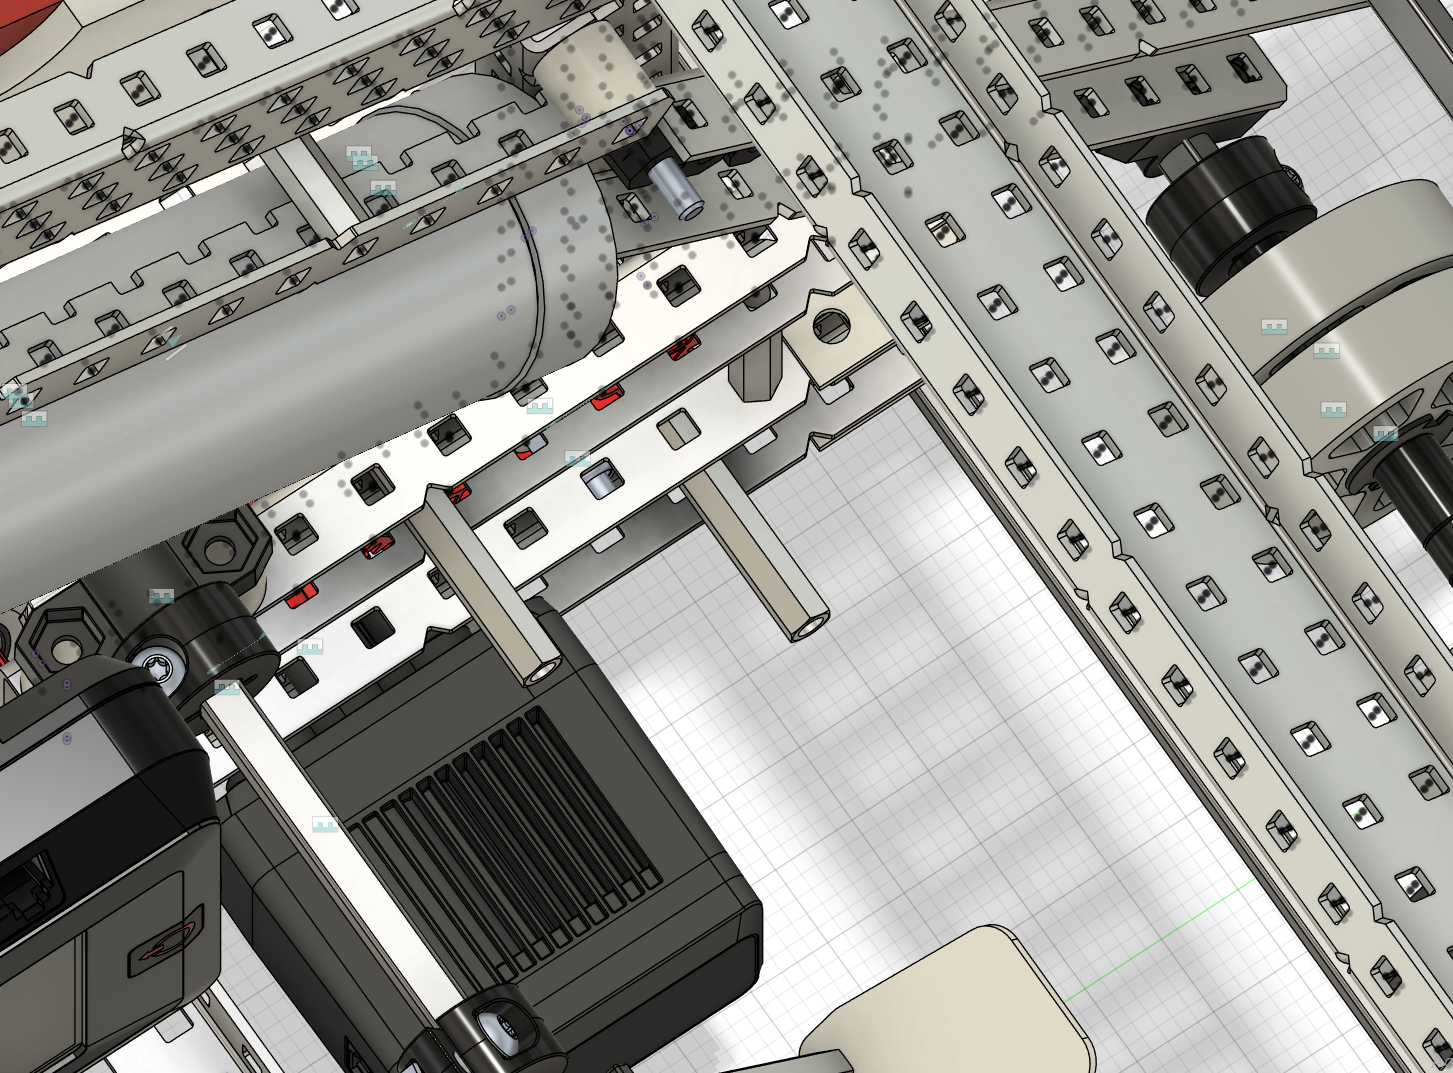
\includegraphics[width=0.5\linewidth]{images/tangentCAD.png}
    \caption{Ramp Mounting}
\end{figure}
considering, also, that the ramp would be forced tangent to the top of the high strength axle running across our drive. It was at this point we decided to revert back to a six motor drive, mainly because we no longer need the extra motor for the Intake, but also because we wanted our drive to have as much power as possible to be as competitive as possible. We simply remove the two 5.5w motors on our drive and replace them with two 11w motors. We placed those where they were before. The next step was to drill holes in our Intake ramp, which was initially made of polycarbonate but we planned to laser cut it out of acetal for more precision, to do this we flexed the ramp tangent to the standoffs and made a mark on either side of each standoff. After drilling the holes at these marks, we attached the ramp using zip ties that went around each standoff. This method was easier, quicker, lighter and more low profile than using screws and it also allowed us more flexibility on where we placed the ramp. Finally, we cut the ramp to length so it was not contacting the floor when the robot was placed on the field. 

\section*{Constructing the Intake}
After the ramp was done we could construct the actual Intake part. The first step was to attach two oversized vertical c-channels, one on either side of the drivetrain. These would serve as mounting points for which the Intake would pivot on. Next we constructed the c-channels that would connect the axle of flex wheels to a motor and mount it the vertical c-channels. These feature a low strength bearing on the middle row of holes at one end and an HS pillow bearing on the other end mounted to the outside flange of the c-channel. 
\begin{figure}[H]
    \centering
    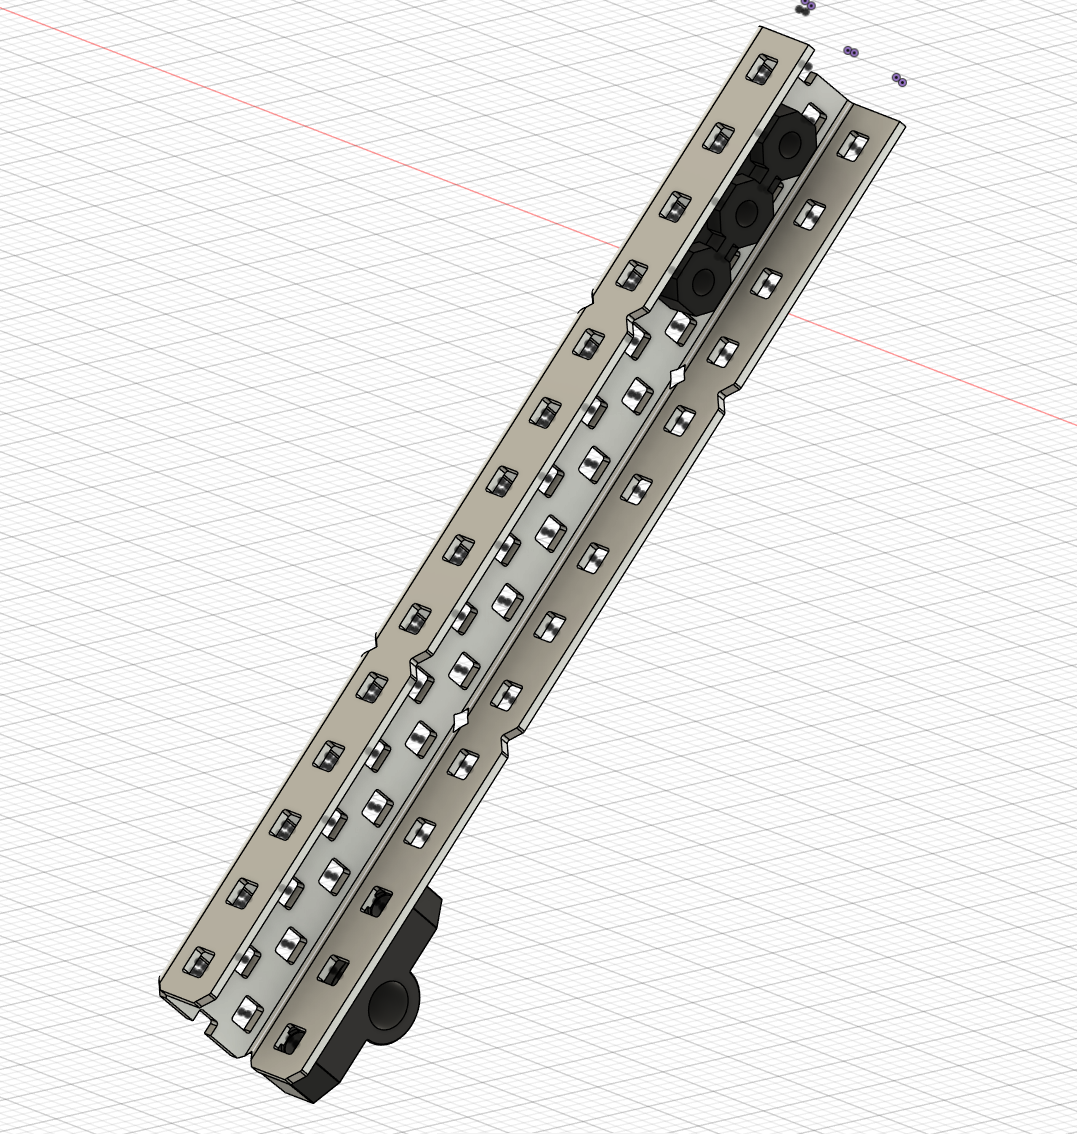
\includegraphics[width=0.5\linewidth]{images/flangecchannel.png}
    \caption{CAD C-channel}
\end{figure}
We connected the two c-channels using a high strength axle going through the two pillow bearings. This high strength axle featured six, two inch, 30a flex wheels and the appropriate spacers and shaft collars to ensure the axle was properly constrained to a width that matches the distance between the two towers. We mounted the motor using a c-channel that was attached to the upper flange on one of the c-channels we had just constructed. This motor connected to the main Intake shaft via 6p chain and two, 8t, 6p sprockets. We used 6p chain 
\begin{figure}[H]
    \centering
    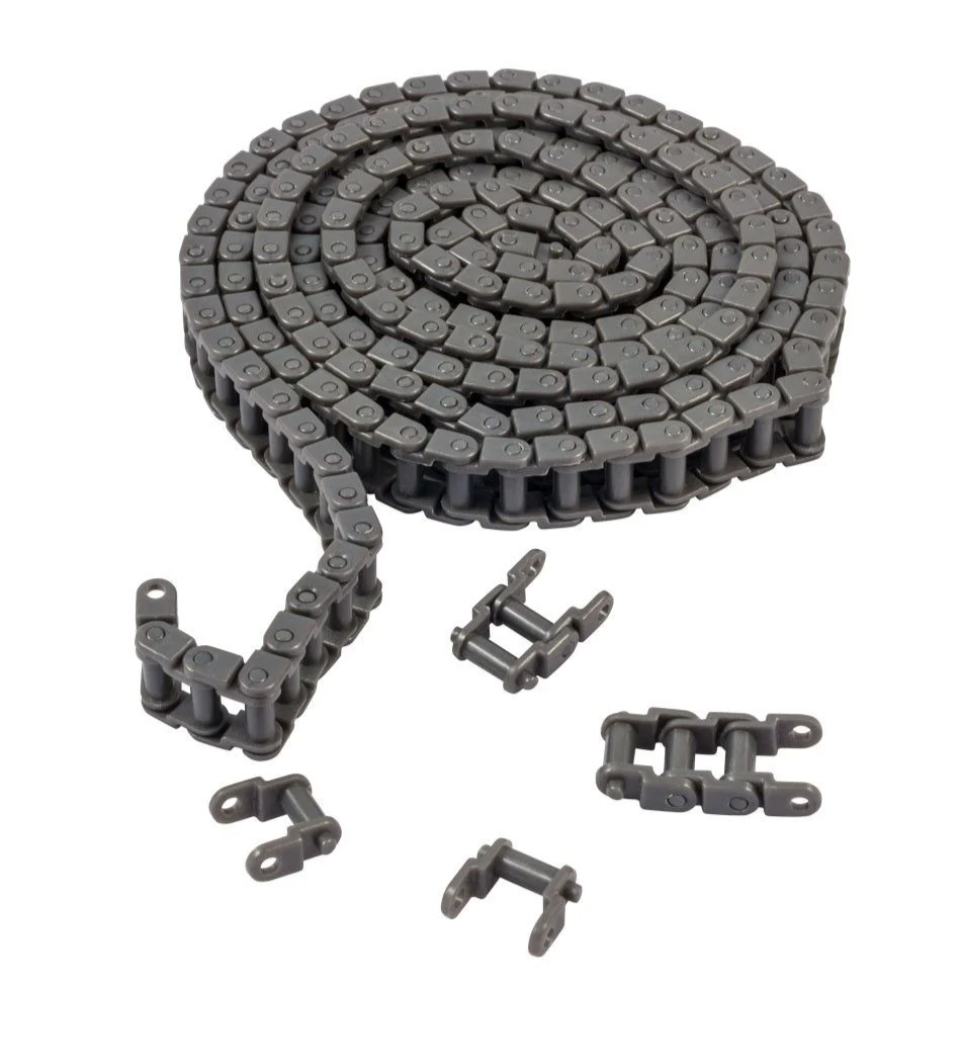
\includegraphics[width=0.5\linewidth]{images/6pchain.png}
    \caption{6pchain}
\end{figure}
because, from our own testing and experience from other teams, we found that it is the most resistant to breaking during use. The 8t sprockets 
\begin{figure}[H]
    \centering
    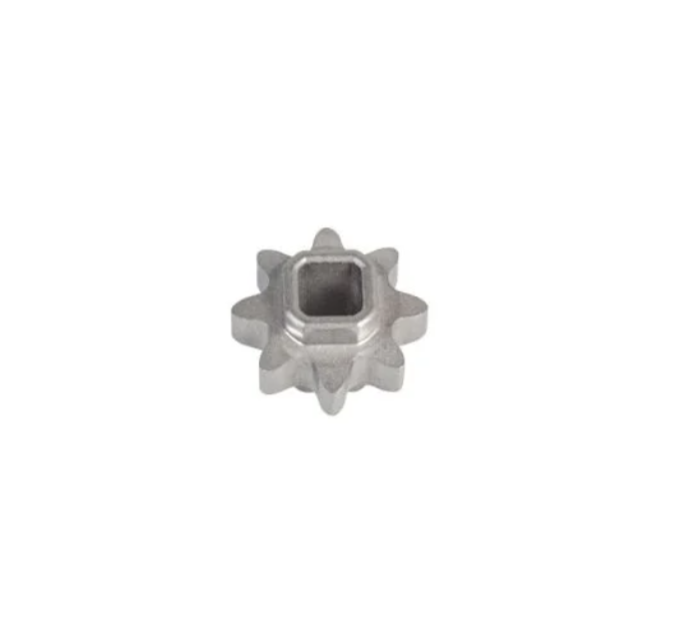
\includegraphics[width=0.5\linewidth]{images/8tsprockets.png}
    \caption{8 Tooth Sprockets}
\end{figure}
were used because of their low profile. The final step was to mount the moving portion of the Intake to the vertical c-channels. To do this we used screw joints because of their rigidity and low friction. Our mounting c-channels served as stoppers to limit how far our Intake could pivot down, so all we needed to do was adjust the position of our screw joints in order to obtain the optimum Intake height. The optimum Intake height is when flex wheels on Intake are low enough so that they can get a proper grip on the Rings but high enough so that the Ring can move past the flex wheel and up the Intake. The final step to our Intake was to add custom Intake guiders made from custom laser cut acetal pieces. These pieces we doubled up on the top and bottom of each side and were connected using standoffs for extra rigidity. 
\begin{figure}[H]
    \centering
    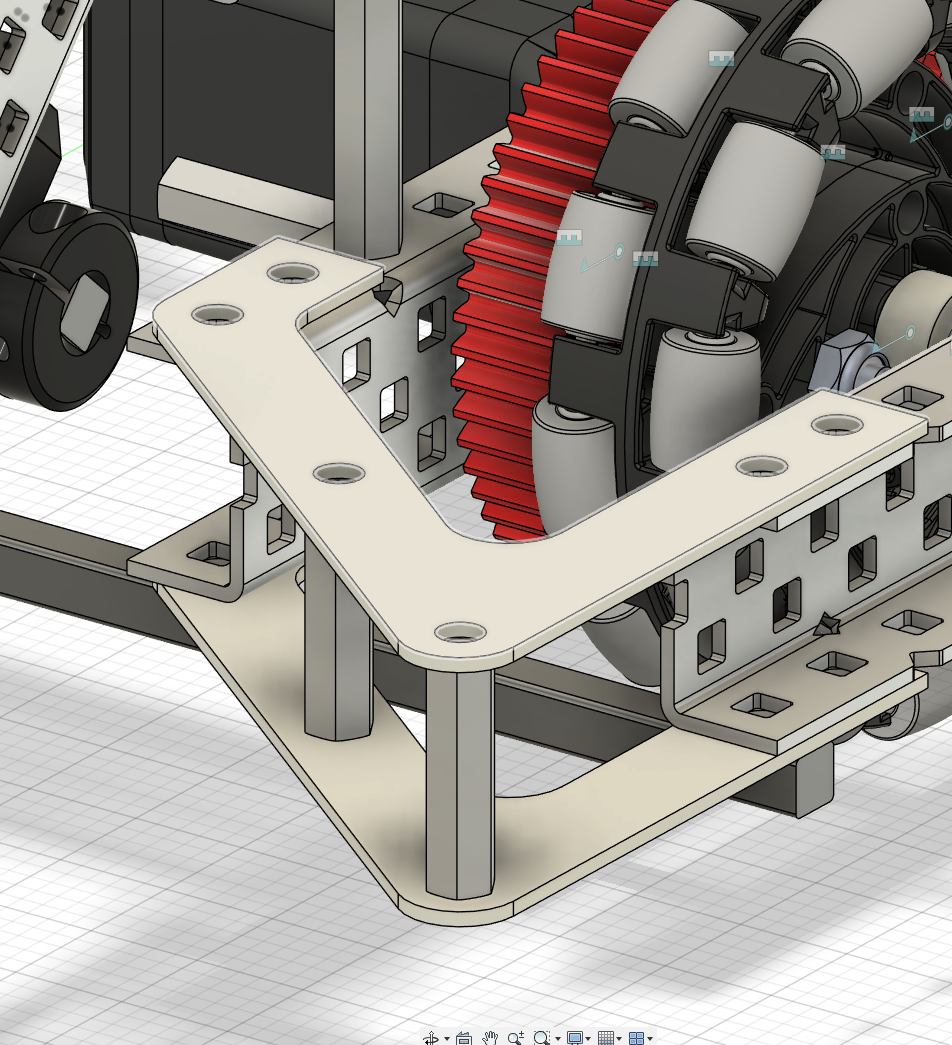
\includegraphics[width=0.5\linewidth]{images/acetalintakeguiders.png}
    \caption{Acetal Intake Guiders}
\end{figure}
The purpose of Intake guiders is simply to guide the Rings into the Intake allowing a wider range of motion that the driver can Intake Rings effectively. 

\section*{Second Stage Construction}
With the first stage constructed, it was time to begin work on the second stage. Our second stage uses a chain with many hooks to hook the Rings from the ramp on the first stage and move them up and flip them onto a stake. This flipping action is the active mechanism we are using to force Rings past the silicon cap on stakes. This is also the same mechanism our previous design used. The first thing we did was mount the top axle and this was relatively easy to do because we simply mounted it at the highest point it could be at while still allowing us to go under the lowest rung of the central ladder, this meant our total robot height was a little less than sixteen inches. This top axle featured a drilled 6t sprocket, secured using the appropriate spacing and shaft collars We wanted the bore of the top sprocket to be circular to reduce friction and, because the shaft it will be on is high strength, the only option was to drill it out using a 5/16 drill bit. This top axle was also oversized because we planned to have our arm pivot on it. The bottom axle needed to be at the same height as the top of the Intake ramp and far enough away so the Ring could fully be Intaken by the first stage before proceeding to the second stage. If the bottom axle was too close to the first stage then there would be a possibility of hooking on the back side of the Ring 
\begin{figure}[H]
    \centering
    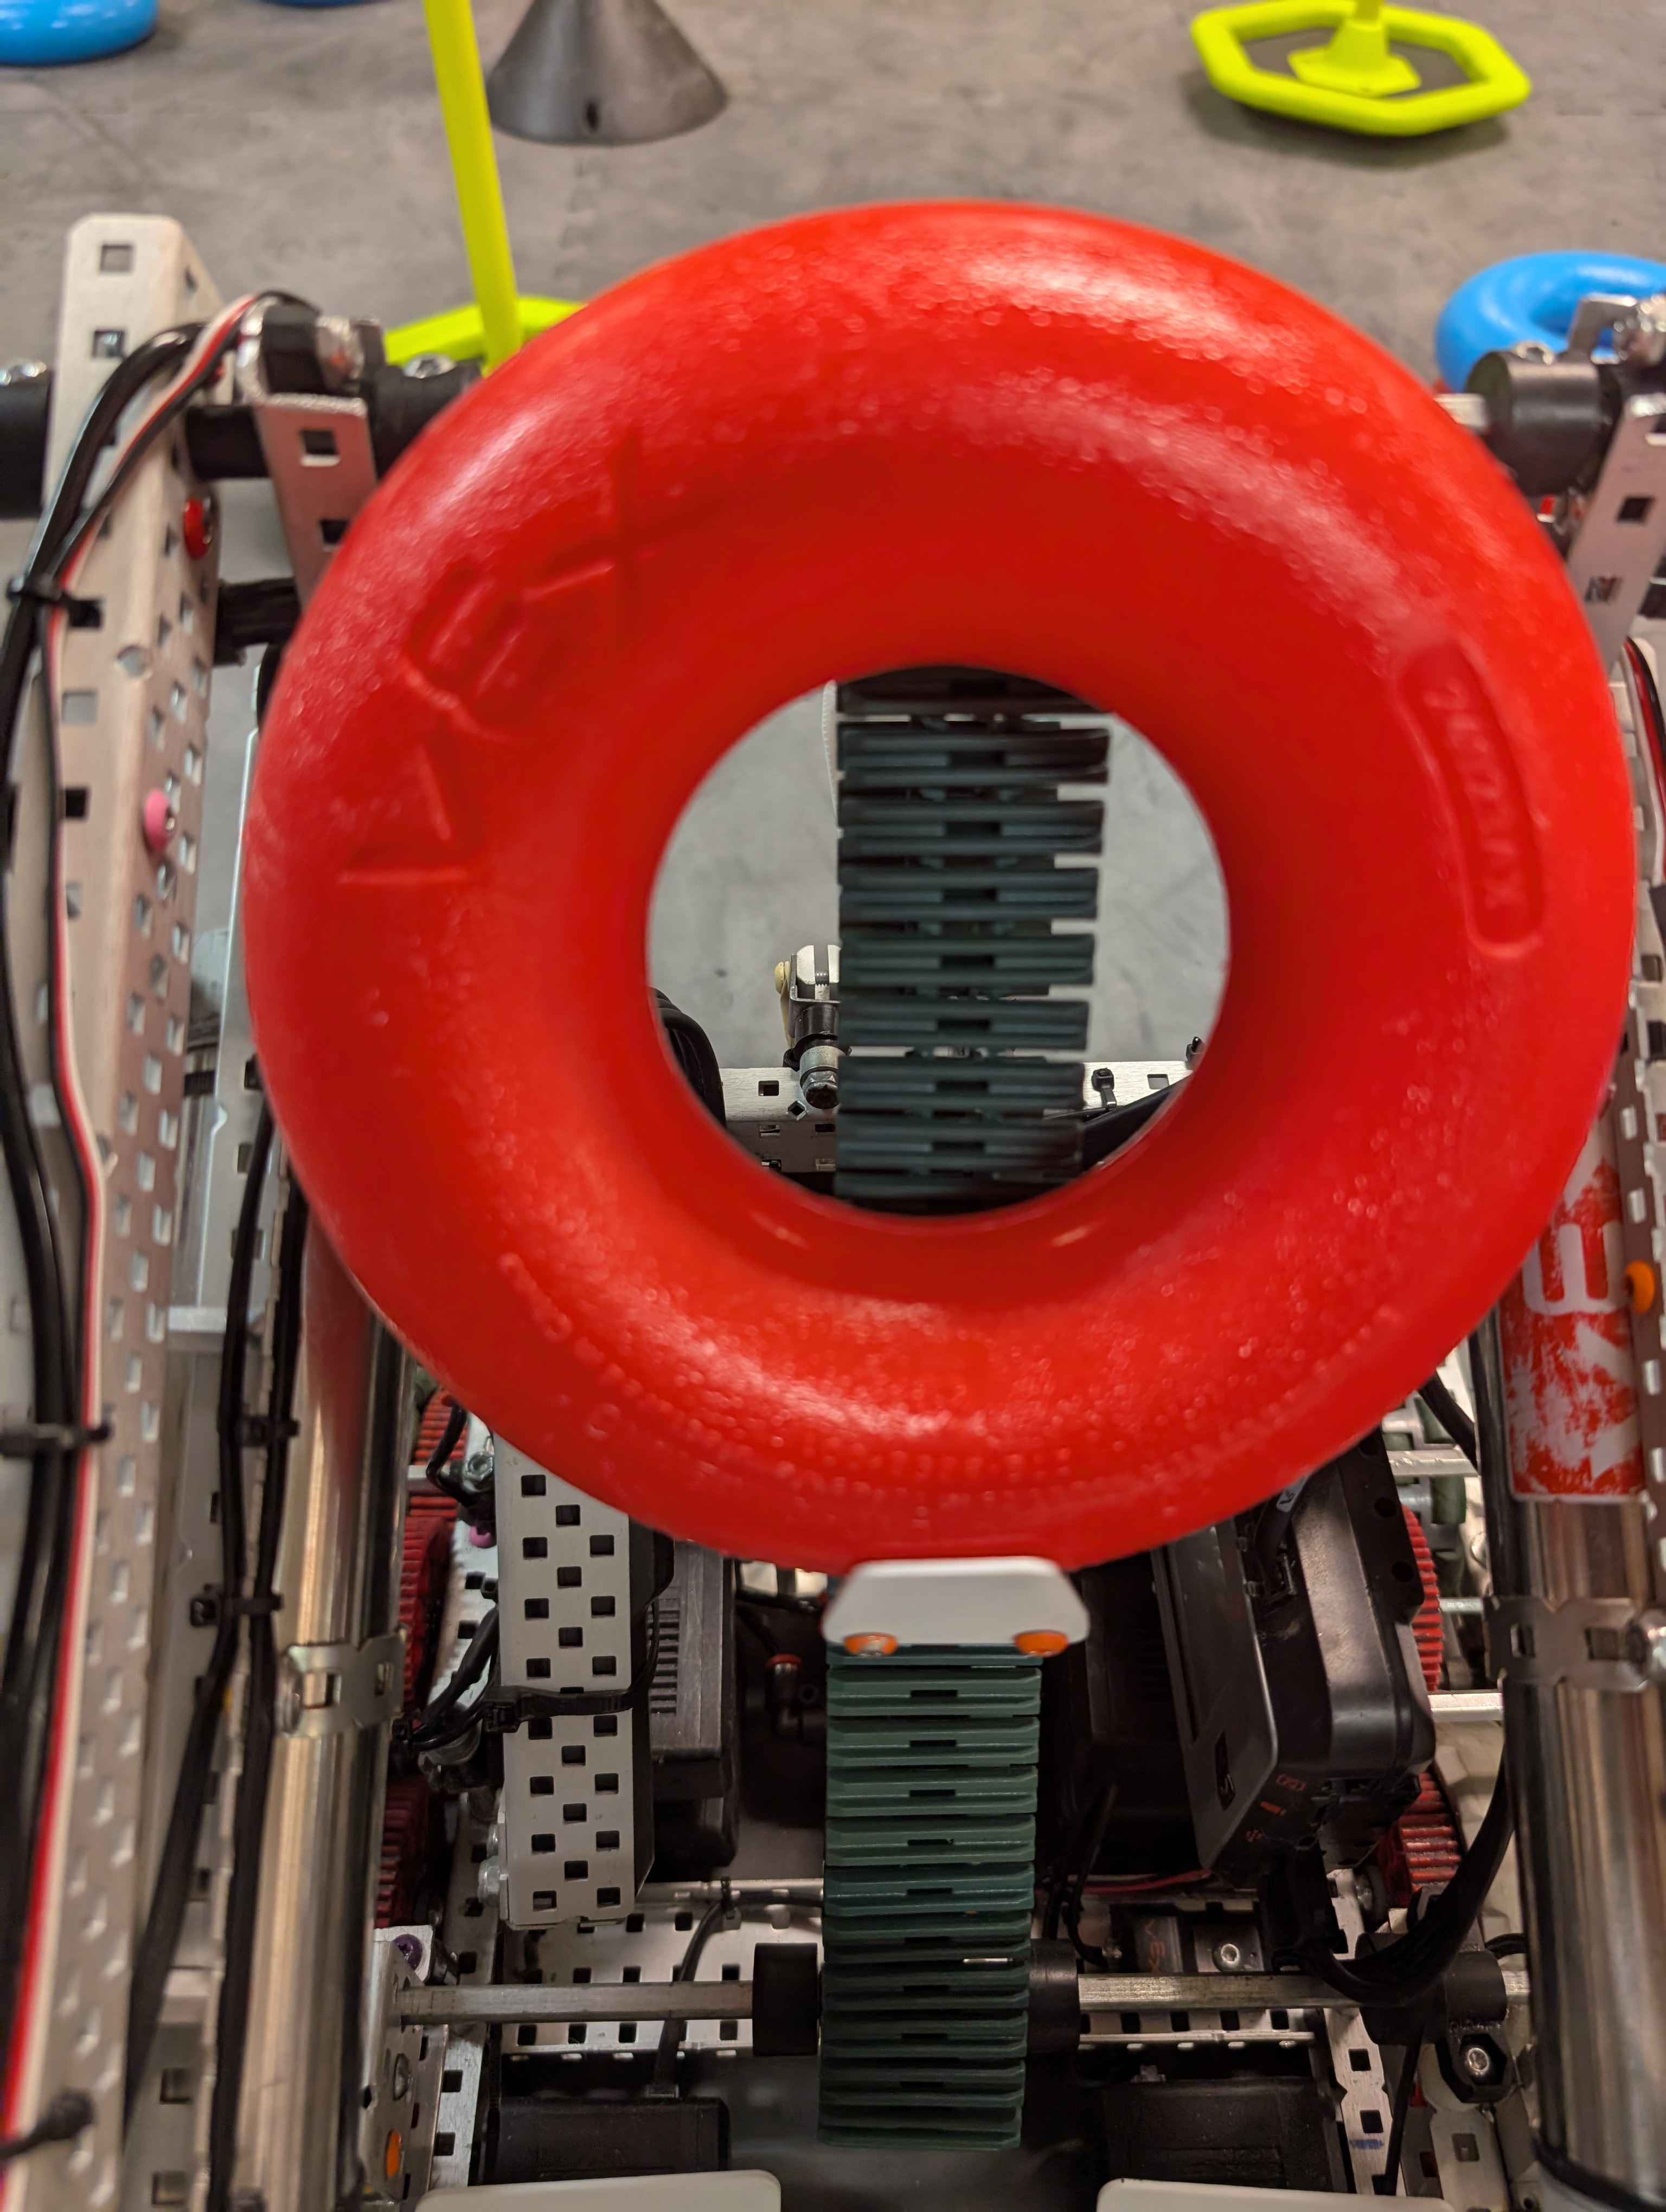
\includegraphics[width=0.5\linewidth]{images/hookbacksidering.jpg}
    \caption{Hooking Problems}
\end{figure}
rather than the inside, preventing our Intake from working properly. After mounting the two axles all we needed to do was attach the same chain we used on our previous design, although adjusting the length to fit. This chain featured a custom hexagon shaped hook attached using two inch standoffs. 
\begin{figure}[H]
    \centering
    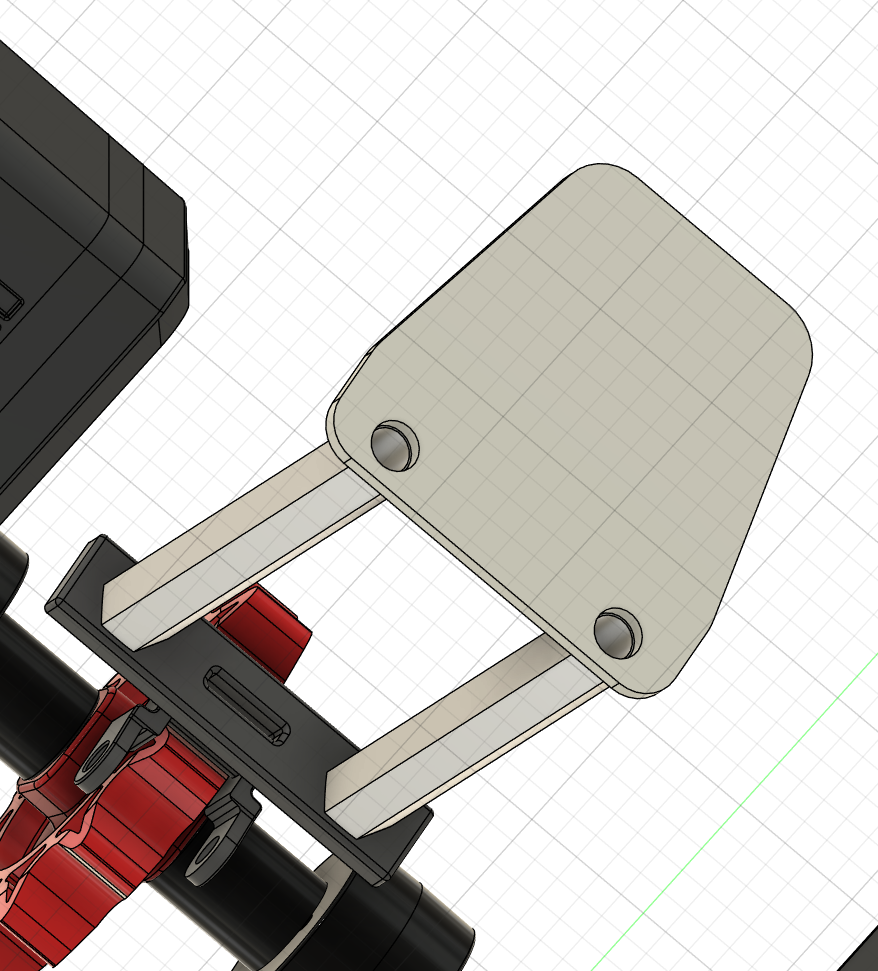
\includegraphics[width=0.4\linewidth]{images/hexagonshapedhook.png}
    \caption{Acetal Hook Connected with Two Inch Standoffs}
\end{figure}

\test{Test the Solution: Intake V1.0 (July 22, 2024)}
\chapterauthor{Caleb Bachmeier}
\info{Caleb Bachmeier}{Test the Solution: Intake}{July 22, 2024}
\textbf{Goal}: Test our built intake solution
\section*{Test the Solution}
Our testing for the Intake will be very simple, can it fill a Mobile Goal completely. We plan to do four different tests each varying nothing. We want to run the exact same four times to see how consistant the Intake is
\renewcommand{\arraystretch}{1.85} % Change this value as needed
\begin{table}[htb!]
\centering
\begin{tabular}{|>{\centering\arraybackslash}m{1.85cm}|>{\centering\arraybackslash}m{1.85cm}|>{\centering\arraybackslash}m{1.85cm}|>{\centering\arraybackslash}m{1.85cm}|>{\centering\arraybackslash}m{1.85cm}|>{\centering\arraybackslash}m{1.85cm}|>{\centering\arraybackslash}m{1.85cm}|}
\hline
\textbf{} & \textbf{Test 1} & \textbf{Test 2} & \textbf{Test 3} & \textbf{Test 4}
\tabularnewline
\hline
Expected Result & 6 Rings scored & 6 Rings scored & 6 Rings scored & 6 Rings scored\tabularnewline
\hline
Actual Result & 5 Rings scored & 5 Rings scored & 5 Rings scored & 5 Rings scored \tabularnewline
\hline
Difference & 1 Ring & 1 Rings & 1 Ring & 1 Ring\tabularnewline
\hline
\end{tabular}
\caption{Intake Testing}
\end{table}
\renewcommand{\arraystretch}{1.85} % Reset to default

This certainly came as a surprise, but we are aware of the reason that the intake cannot score more than five Rings, the hooks on our Intake get caught on the fifth scored Ring as shown in \ref{fig:intakeproblem}
\begin{figure}[h!]
    \centering
    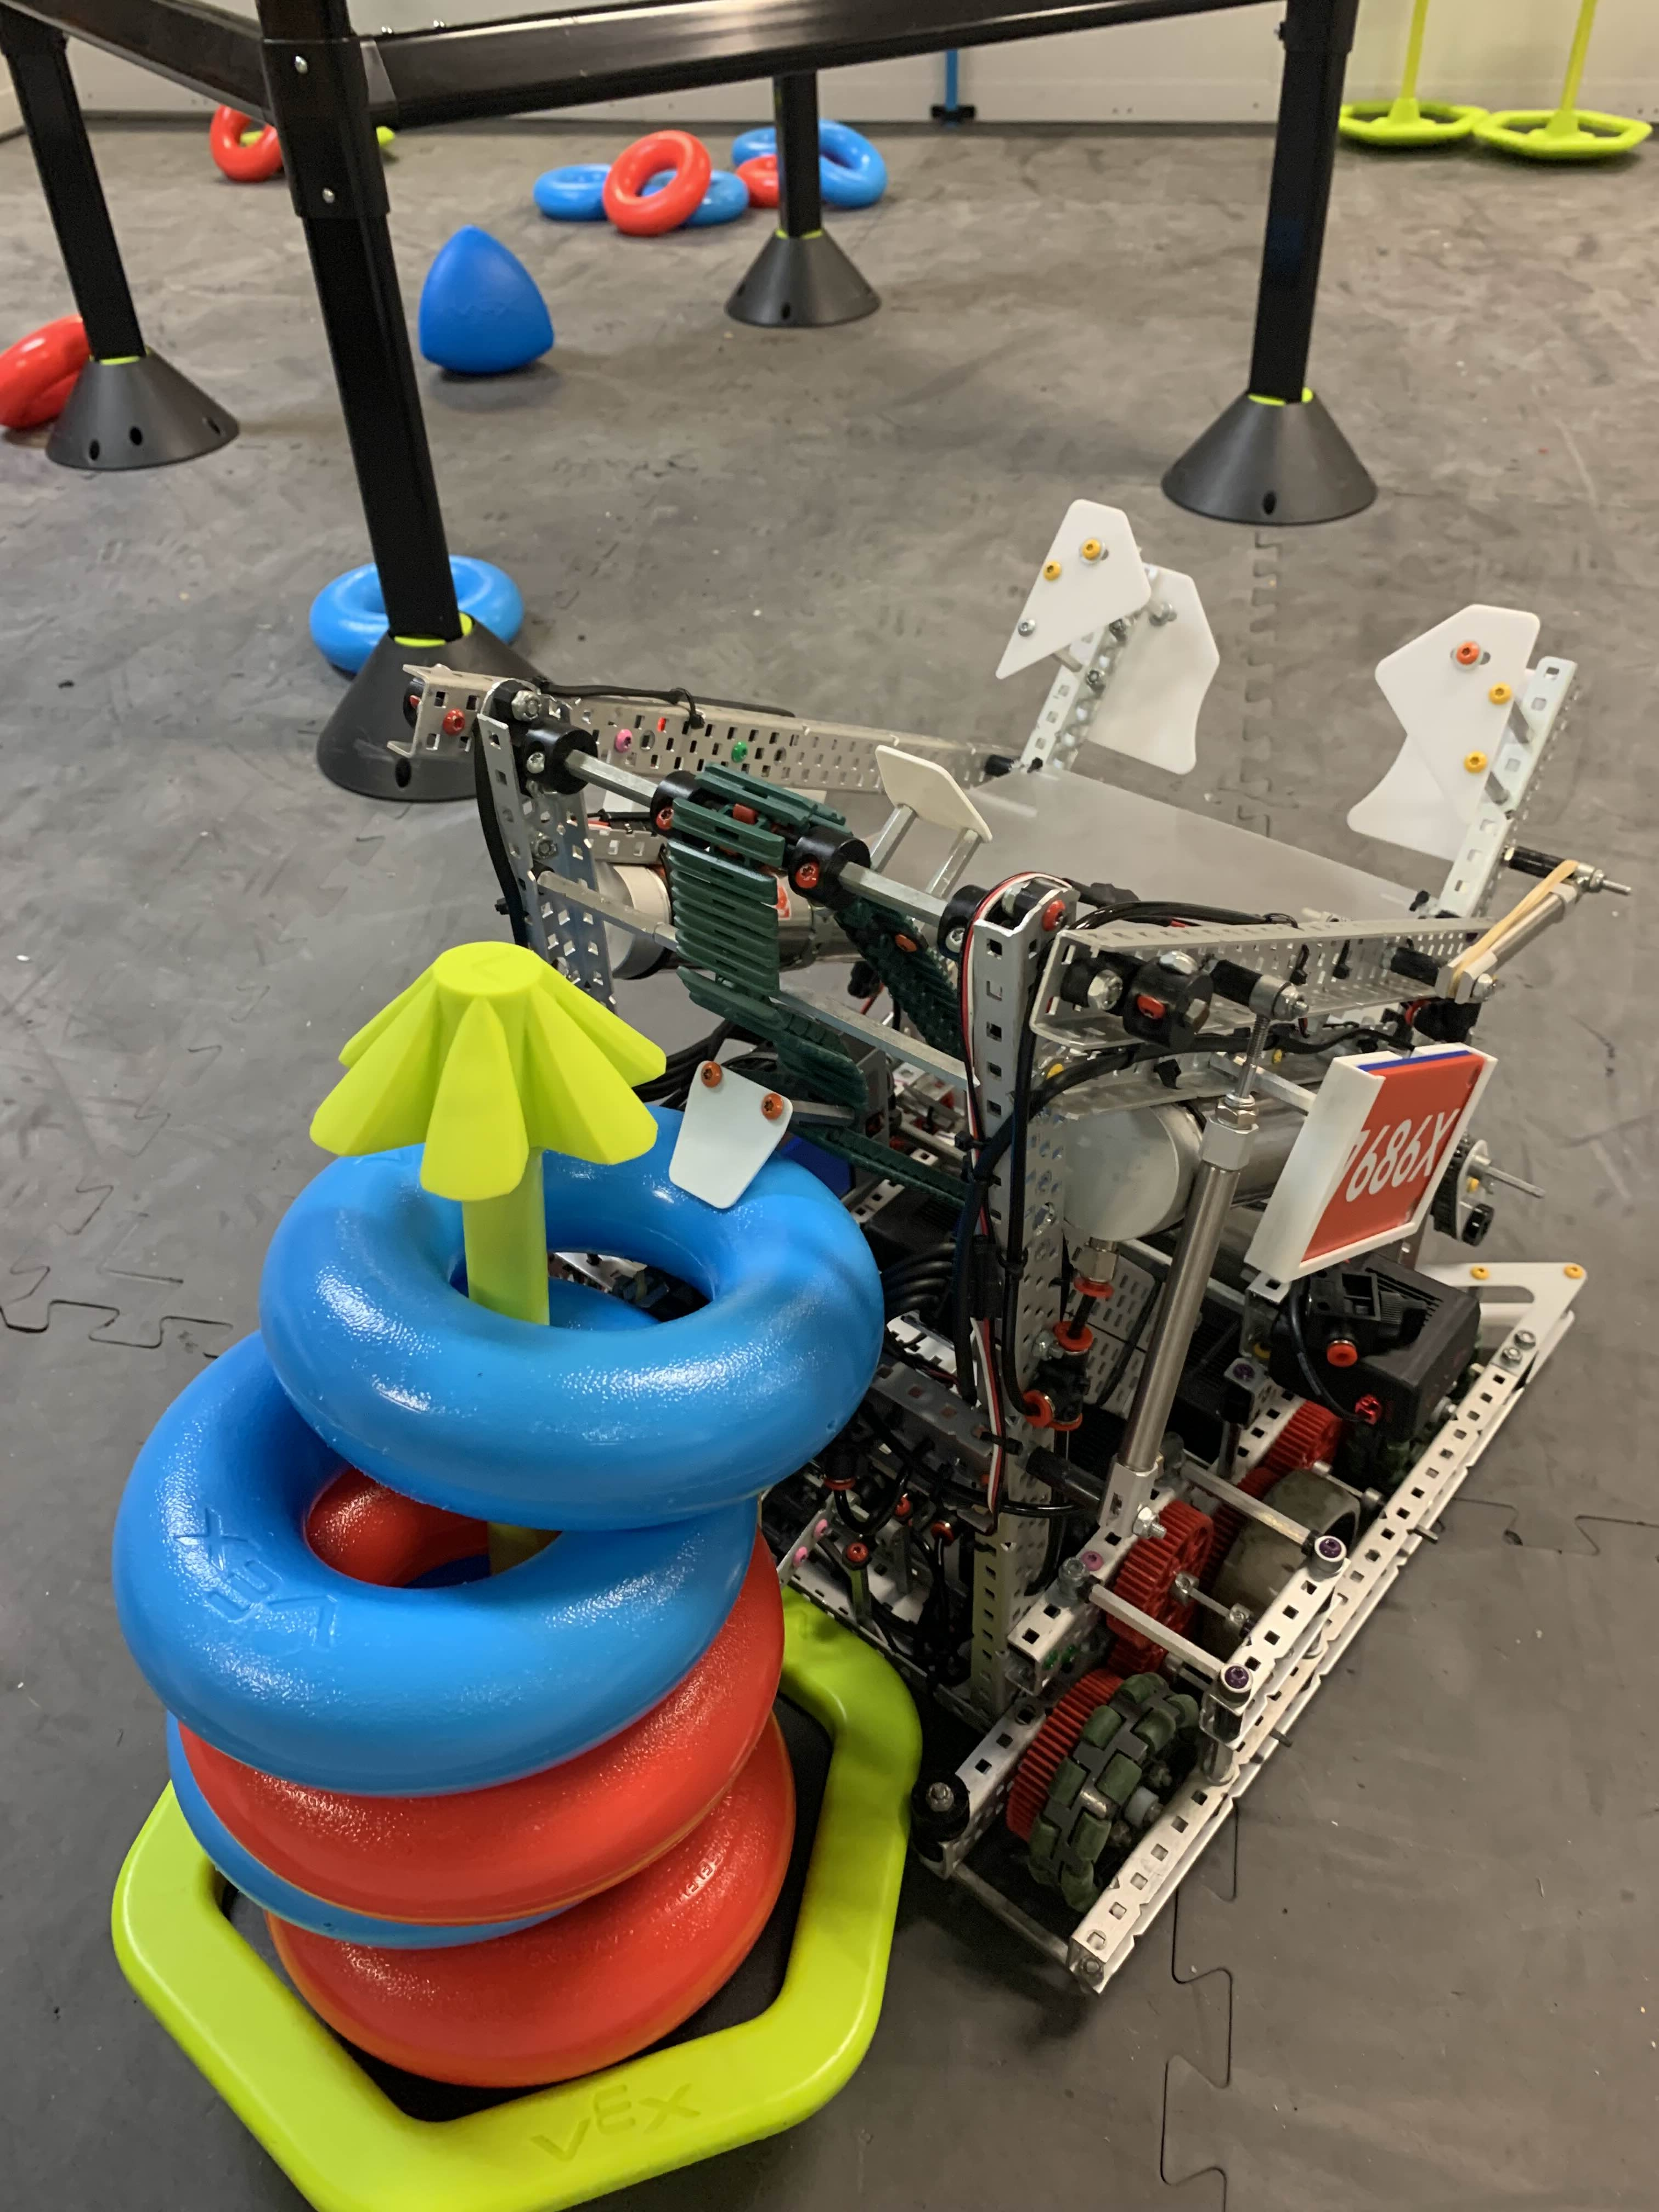
\includegraphics[width=0.5\linewidth]{images/Intake-problem.jpg}
    \caption{Our intake problem}
    \label{fig:intakeproblem}
\end{figure}